\startchapter{The Problem to be Solved}
\label{chapter:problem}

\newlength{\savedunitlength}
\setlength{\unitlength}{2em}

A number of neurological disorders can leave a person with diminished ability to communicate and function in the world.
Individuals with Parkinson's Disease, Amyotrophic lateral sclerosis, or individuals locked in syndrome\cite {} fit in 
to this category.
The standard set of interaction tools that a human uses to interface with the world requires our brains to generate 
the correct gross and fine movements to complete an action.

It is possible to gather the signals that the brain makes to initiate action planning and execution of movements. 
There are a number of methods for this ranging from noninvasive to subcellular alteration. Every method has its drawback.  

Optogenetics - Invasive injection that requires you to add genes and alter your brains genome. Invasive addition of 
hardware to read out the signals.

Microelectrode array\cite {}Is a set of electrodes that is set up in a pattern, usually a two dimensional grid, 
that is implanted into the brain. MicroElectrode arrays have the advantage of being able to record in both high 
temporal and spacial resolution. With this high temporal and spatial resolution it is possible to determine the 
patterns of firing that correlate with the aspect of movement. Local Field Potentials give the electrodes access 
to neurons in a volume of \cite {}.

Positron Emission Tomography\cite{} (PET) - Is the the use of an injected radioactive analog of a biologically active 
molecule\cite{}, coupled with gamma ray detectors to detect the metabolic activity in a tissue. When scanning the 
brain areas that are actively processing information exhibit greater use of resources. The use of the radionuclide 
is the connection between the activity of the brain and the detection of the gamma rays. Problems with such a system 
is that they are relatively large uses a ring of  photomultiplier tubes. Also requires a computer tomography scanner 
to correlate with the users individual cortical structure. Radiation from the radionuclide while coming from a short 
lived radioisotope is still able to cause cellular damage. A system like this would not be a suitable for long term 
use as a brain computer interface. Lower spatial resolution due to the positron traveling through the tissue of 
interest until it collides with an electron.

Functional Magnetic Resonance Imaging\cite{} ( fMRI ) - uses Magnetic resonance Imaging\cite{} which uses a large
magnet to polarize all the spins of the electrons[citation] of an atom. A smaller magnet is used to resonate an 
atom of choice by using an appropriate resonant frequency. This causes an emission of a radio signal that is recorded 
and interpreted by a computer. The computer then creates an image of the locations of the emissions of the radio signal 
which corresponds to the structure of material in the scanner. fMRI uses the Blood Oxygen Level Dependant\cite{} ( BOLD ) 
signal to detect where activity is occurring in the brain. The BOLD signal  is a measure of the difference between 
the oxyhemoglobin and deoxyhemoglobin. As in PET where neurons use the glucose and have to uptake more when they are 
active, In fMRI the neurons are using their oxygen and uptaking more from the blood. There is a difference in the 
magnetic susceptibility of the proteins. This difference can be measured and this gives the location of the activity 
in the brain.

The problems with fMRI for a BCI are: The scanners have to be fairly large. This is due to the primary magnet of an MRI 
being large enough to generate a sufficiently powerful magnetic field. due to the magnetic field being so strong the 
area that the magnet is housed in has to be free of materials that could interfere with the magnet or could attract 
the material with catastrophic effects on the magnet. The radio signals are also relatively weak so electromagnetic 
shielding is needed to get the best results. The temporal and spatial resolution are one second resolution, one mm 
voxels. Some signals can be used to determine the mental state \cite{}[This paper ] of a user which in turn can be used to 
control some forms of BCI [This paper 1, keyboard].

Electrocorticography\cite{} ( ECog ) - require electrodes to be implanted on the brain itself. A craniotomy is needed to 
gain access to the brains surface. resolution is better than EEG. The signal to noise ratio from the signal is better.
Signals are stronger as they are not being read through the skull and other tissue between the brain and the 
electrodes.

Electroencephalography\cite{} ( EEG ) - drawbacks -signals are overaged from areas of the brain, not many electrodes, 
signals in sulci not expressed well in the reading 

Signals from neurons are recreated from the combination of the signals that reach the electrodes through the skull. 
This can lead to a limited amount of spatial resolution \cite{}[ 2 ]  )

Problems with sampling could occur if the placement of electrodes was not correct when implantation occured. 

higher signal to noise ratio.

For humans to have a greater merger with their machines, methods that allow for fast accurate interaction must be 
developed.


\subsection{Research Question}
frame the question

ask the specific question


\section 3
\subsection {name}
There are a few different ways to learn of the state of the mind one of which is the Electro Encephalograph. 
This is the measurement of the electric fields on the scalp. These electric fields are the combination of of the 
fields from the environment and the brain. External fields are generated from the electronic equipment that humans 
have created that is not shielded. examples are the Radio waves from any number of transmitters to the the sixty 
hertz noise generated from the power transmission system.

Electrical fields from the brain are generated from the collective activity of the axons in the brain(and maybe the quantum fluctuations of the ).  <todo> more detail if needed </todo>

the resultant signal that the EEG detects is one that is created by the synchronous firing of many cells 

Activity bands\cite{}

Artifacts - electromyographic\cite{},
kappa rhythm - eye futter artifact

electrodes settling can cause popping artifacts in the readings, 

activity from the local electrical grid 60 or 50  hz.

iv drips can cause artifacts too - not a problem with my study


\subsection {Artifact removal: independent component analysis}


\subsection {Interpretation of brain activity}


\subsection{Emotiv EPOC}
The Emotiv EPOC is commercial wireless electro encephalograph. It has fourteen electrodes which means 14 channels 
of data. The electric field of the scalp is sampled 128 times per second.

One of the ways that researchers using EEG keep their experiments replicable is through the use of standardized 
electrode placement. One of the standards is the 10-20\cite{} system INSERT IMAGE.
The location of the electrodes in this system are based on percentages of the distance from either the front and 
back of the scalp or the right and left side. The 10-20 locations for the emotive are 
af3, af4, f3, f4, f7, f8, fc5 , fc6 , t7, t8, cms, drl, p7, p8, o1, o2[ ref ].

The EPOC can function in few different ways cognitively, affective, expressively, and positionally.

It has the ability to discern a few cognitive states,

The EmoEngine analyses that data collected while the user is performing tasks on a cube that is displayed on screen. 
The data is the collected brain waves from all the channels. This data is then analyzed (HOW?) and classifications 
built for the thirteen possible actions a user could do with the cube. the actions are the 6 directions of movement, 
six types of rotation and the ability to make the block disappear. Once the user has trained the EmoEngine on the 
states they can assign actions to the states. With these actions the user can then interact with the computer via 
their thoughts.

Affective states are detected by general frequency [ ref ] of the electrical activity detected by the electrodes. The specific powers of the frequency bands have been identified and correlated with specific affective. affective states that can be detected are engagment, instantaneous excitement and long term excitement[epoc manual].
Many of the electrodes, especially thoughts nearest the face, receive large changes in voltage when the muscles of the face activate. These voltage changes are used to sense the facial muscles, from this the expression of the user is classified and thus the expressive state of a user.
The EPOC�s two dimensional gyroscope allows for the position of the users head to be used as input as well. The most used controls linked to the gyro are used for head position tracking or mouse control.
The EPOC headset also has built in wireless communication with the host computer. This allows for more freedom when the user or subject is wearing the headset as there are no wires to hinder them.

The procedure to use the Emotiv EPOC is as follows.
Insert electrodes by twisting them into their slots.
Wet the felts on the electrodes with a saline solution of concentration 0.154 mols per liter[ ref ]. A common solution is contact solution or saline solution found in a pharmacy. Once the electrodes are wetted, open the Emotive control panel program. In the headset setup tab there is an image of a superior view of the human head. There are a sixteen circles on the view that will be red.
The red dots indicate the state of the electrodes and the connection. Black is no signal, Red is a very poor connection.Orange poor connection and yellow is a fair. Green means that the connection is good and the signals from the brain will be strong.
Place the EPOC on the head and fit it snug with the reference electrode on the temporal bone behind the ear.
The solution in the felt pads on the electrodes improves contact with the scalp and allow for better conduction of the electric field to the electrode. Sometimes the hair of the user gets in the way and due to capillary action on the hairs surface the water moves from the electrode along the hair. If this happens it can be necessary to replace the solution in the electrodes and place head set back on the head. The user or technician can tell if the headset has a proper connection to the scalp with the Emotiv control panel. When the circles turn green then the signals can be received.


\subsection{My program }
I wrote a program that receives the recorded values from the EPOC headset and saves them to a file along with some of the users actions. The actions I record are . I recorded the key presses and the mouse movements with User32.dll in a windows 7 computer. I also recorded the user head movements with the built in gyros of the EPOC headset. 

\subsection{user32}
Windows USER  is the general name given to the section of the windows operating system that receives, uses and creates interfaces with the user. The implementation of this is in the dynamic link library user32. In 64 bit versions of windows there is a modified version of the user32 

With the P/Invoke a program can hook the functions in user32. Using this the program can collect the following data from the mouse. Right and left mouse click, up and down on the mouse wheel as well as the position of the mouse on the screen.
From the keyboard the data collected is all the keys for letters and numbers are collected. The shift keys cap locks tab alt, left windows, apps, numlock, 

The recording of the control key was missing in the original set of data that I collected. After looking at the data it was noticed absent and added into the program. No new data has been collected with the control key recording. 

The absence of this key is of no concern at the moment. If it is possible to train the artificial neural net to recognize most of the other recorded classes it would become useful to get more data with the control key and train a recognizer for the control key.

HOw the FielLE wAS saaaved?binary vs txt

\subsection{Preprocessing of data} [ Data Mining paper ]
For a test of data mining with WEKA and its built in neural networks, we attempted to correlate the EEG data with the direction the mouse was moving. I used the data of the mouse position and found the cardinal and intercardinal directions of the movement. To find these directions the deltas for the x and the y were found. The arctan function was used to get a measure of the angle of the vector the deltas formed. The angle of the vector was then rounded to the nearest cardinal and intercardinal direction of the compas. The rounding was done based on the division of the circle in to 22.5Degree segments.  
    The deltas that were chosen, were based on the amount of time the mouse was moving. This time was related the time between line writes in the data. If the mouse had not moved in 30 lines of data then a mouse movement was considered to have stopped. If the data for a detected mouse movement was very long I decided to stop it at 188 lines as most of the movements examined in the raw data were smaller than this number of lines.

The second of data before the mouse movement started  used for training the WEKA neural network. The reason for this is based on studies from Benjamin Libet�s work in the 1970s.
Libet used EEGs for his experiments, his subjects wore then will they were told to press a button or extend a finger. Libet also told them to watch a timer, when his subjects became aware they wanted to press the button or extend a finger they were to note the time. This allowed the the researchers to look at the EEG for a signal that would correlate with the button press. After analysis Libet found that the participant reported the urge to act at 200 milliseconds(ms) before the button press, with a margin of error of 50 ms. The EEG showed that there was a rising potential 500ms before the button press. This means that there were 300 ms before the execution of the action that the brain showed signs of initiation of the action. This means that after a about a third of a second the user becomes aware of an action that the could execute. 
Daniel Dennett�s comment was � the action originally  precipitated  in some some part of the brain, and off fly the signals to muscles, pausing en route to tell you , the conscious agent what is going on �. More modern fMRI studies show similar findings with regions of the brain activating before the action was executed[ ref ]. 

IMAGE FOR LIBETS EXPERIMENT
\begin{figure}[h!]
\centering
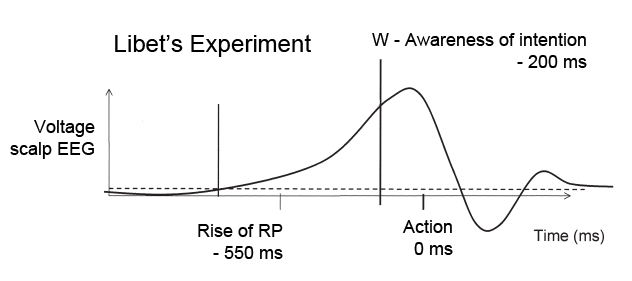
\includegraphics[width=0.9\textwidth,natwidth=632,natheight=281]{./Figures/LibetExperiment.png}
\caption{LibetExperiment}
\end{figure}

[ ref ][ ref ]
With the fact that there is measurable data from an EEG to discern that movements are coming it would be a minimal feature to look for in the data from the EPOC.

\subsection{Put this some where}
Tried both direction based and raw data(say it wasn't just the second before the event) for the Naive Bayes, Bayes net and Multilayered perceptron in weka.

\section{Artificial neural nets:}
- [introduction to Neural networks in c\#] -
number of hidden layers
layers
none - only capable of representing linear separable functions of decisions
one - can approximate any function that contains a continuous mapping from one finite space to another
two - can represent an arbitrary decision boundary to a arbitrary accuracy with rational activation functions and can approximate any smooth mapping to any accuracy
one hidden layer is practical for most any function
there is no theoretical reason to go to more than 2 layers 
the number of neurons in the hidden layer
underfitting - too few neurons in hidden layer
not good for a complicated data set
To many may result in overfitting
limited information is not enough to train all the hidden layers neurons
sufficient info - to many neurons - too much training time.
Rules of thumb
number of neurons between the number of output and input neuron number
hidden neurons 2/3 size of input plus number of output
number of hidden neurons less than twice the size of the input layer
You will have to ultimately try various numbers of Hidden neurons - kurzweil says evolutionary algorithms.
this can also give you specialized neural nets that may be better for some but not other applications.

IMAGE OF CORTICAL COLUMN

\section {Real Neural Networks}

Information processing in animals is done with networks of neurons. In vertebrates its done in large networks of neurons called brains. Humans have an advanced brain capable of simulating the environment and planning for the long term future. 

What is the brain
    The brain is a approximately 1.5kg mass of information processing and support cells. The brain is composed of many different structures. Cerebellum is a largely repetitive structure primarily used for motor learning and fine control located at the base of the brain. Brainstem consists of a few sub regions. At the top of the spinal cord is the Medulla oblongata which contains many of the automatic functions to maintain homeostasis such as heart rate, and breathing . Above the medulla is the Pons which has white matter tracts to move information to and from the body. The pons also has some regulatory functions such as helping control the muscles of the face, eyes and throat, equilibrium, hearing and taste and facial sensations. The last region in the brain stem is midbrain � vision, hearing, motor control, sleep/wake, arousal (alertness), and temperature regulation.[2]�. 

The Thalamus is a region of the brain above the brainstem.
Limbic .
Cerebral cortex .
The Cerebral cortex is divided into four main lobes. The occipital, parietal, temporal and frontal, 
White matter .
Grey matter .

\begin{figure}[h!]
\centering
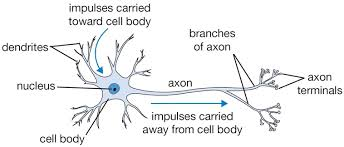
\includegraphics[width=1.4\textwidth,natwidth=535,natheight=308]{./Figures/Neuron.jpg}
\caption{Basic neuron}
\end{figure}
IMAGE OF NEURON

The brain is made up of two types of cells Glia and Neurons are the main cells of the brain. Neurons are the main information processing units of the brain, with glia being an important partner cell to neurons. As they help to maintain the environment for neurons and help regulate synaptic connections. Neurons have some specializations that allow them to process information and pass the new information to any neurons that are connected to them. The specializations are the Axon and Dendrites. Axons are extensions from the Soma starting at the axon hillock.There primary purpose is to carry an action potential to the synaptic boutons. Action potentials will be discussed in more detail below. The axons can be myelinated or not by special glia. If they are myelinated they have a better conduction speed. This is due to the ability of the myelin to allow the voltage to be transmitted via saltatory conduction. The action potential is thus conducted past the section of the axon that is myelinated and to a section of the axon that is not myelinated. This unmyelinated section is called a node of Ranvier. At nodes of Ranvier the action potential is regenerated via the ion channels present in the cell membrane. If there are the axons are entirely non myelinated then the action potential is entirely transmitted with ion channels. 
Synapses occur between two neurons and are the location where information is passed from one neurons axon to its neighbors Dendrites. The synapses work either with a chemical or electrical connection[gap junction]. Chemical connections being the most common in vertebrate brains[ ?REF? ]. Chemical synapses work by the following mechanism. When the action potential reaches the location of a synapse it triggers neurotransmitter release. the voltage change from the action potential in the membrane opens up the local Ca+ ion channels. As the Ca+ ions build up in the synaptic bouton the Ca+ binds to the two binding sites on synaptotagmin.  vesicle(VAMP vSNARE), target membrane(syntaxin, snap25, tSNARE) [ snare complex ]
[ ref ] [ molecular mechanisms of neurotransmitter release ]

Dendrites are 
     the postsynaptic terminal 
    dendrites work to sum the incoming information of the connected synapses.
    
how spikes are generated, 
    Action potentials
        voltage gated ion channels
how signals are transmitted 
    chemical 
    gap 
networks in the brain 
    columns
top down processing 
bottom up processing


Human brain < i guess this should be in a discussion about ann and how they compair with the human brain.>
~100 Billion neurons
~100 Trillion synapses
~300 Million minicolumns.
~80-120 Neurons in a minicolumn
~1000-10,000 Inputs/cell
~700 New neurons every day [ ?ref? ]

\section {Liquid State Machine}

separation property a measure of the euclidean distance of the states of the network with different samples. 
%http://www.phil.uu.nl/preprints/ckiscripties/SCRIPTIES/067_matser.pdf
also good at approximation


4. Make it exciting, make it current, make it important - why do I want to keep
reading?
Why is it current?
Brain Computer interfaces are coming of age. The work of Miguel Nicolelis.
One of the issues with brain computer interfaces for humans though is that they would require an invasive procedures. Some could be optogenetic (I think this is the most promising) or micro electrode array. The procedures for these technologies have potentially adverse health effects. These health effects range from inflammation around areas where surgery was performed to death. anytime you have major surgery you have the potential for death. optogenetic interfaces in adult animals

Why is it new?
Its new because it uses a liquid state machine in the configuration of the mammalian auditory system.
the use of a fourier transform for the first part of the processing is ?unique. (<todo> has this been done before</todo>). this should allow for more modularity in the structure of the lsm. it is also closer to how natural systems have come to good solutions for the processing of data that is frequency based and spatial temporal.



5. Should you list here the solutions from other researchers? I think not, list
instead the different facets of the problems that other researchers have attacked.
:facets - 



6. A taxonomy can be extremely useful to place your problem and its particular
special features within the perfect context of the overall area, as you need to
make sure that the reader understands perfectly what you are trying to solve.








\setlength{\unitlength}{\savedunitlength}
